\chapter{Prosessdokumentasjon}
\marginpar{
Test for sitering av kilder.\cite{forelesning:tulpesh}\cite{book:utforming}\cite{book:desintsystems}
}
\lettrine[lines=2]{I}{} følgende kappitel beskriver vi hvordan hele utviklinsprosessen for protitypene har foregått. Hensikten er at man skal illustrere hele prosessen fra idé, mockup til hi-hi prototype klar for brukertesting. Kapitlet består av mange for å på enklest muli måte ilustrere prosessen. for eventuell beskrivelse av funksjonalitet av de inngående moduler som er synlige på bildene henvises til appediks \ref{app:funksjonalitet}.




\section{Første utkast}
\marginpar{Viktige prinsipper:
feedback, constraints (bruker får ikke gjøre feil), affordances
}
\marginpar{Støtteord:
Usability (brukbarhet): konsistens, brukerkontroll, passende presentasjon.
}
Etter at idéen om hva vi skal jobbe med var klar og diskutert tok det ikke lang tid før vi ble enige om hvordan vi skal sette sammen vårt forslag til en helhet. Hele gruppen var tydelig på at vi ønsker i stor gra å benytte oss av en løsning som baserer seg tydelig på gestalt prinsipper.
Det som var spesielt viktig var at man deler opp de forskjellige moduler i flere undermoduler slik at de bilder en visuell og logisk helhet. 
Forslaget var ganske klart opplegg der alle viktige moduler blir satt asmmen i en overordnet gruppe som disse tilhører. I det første utkastet bestod disse av:
\begin{center}
Editorer | Meldinger | Resurser | System | Servers
\end{center}
Dessa skulle plaseres på en velkomstside som innholdr også annen viktig informasjon for brukeren. Man skal bli presnetert med sin brukerikone i øvre høyre hjørn pg en hurtigtilgang til systeminstillinger. Under skal det også eventuelt presenteres noen <<widgets>> som viser systemstatus, påloggede bruker, andel brukt ram-minne, tilgjengelig lagringsplass og kjørende prosesser. Alt dette blir pakket ned til en dynamisk nettside og vil være tilgjengelig via en webbrowser.





\begin{figure}
%bruk \begin{figure}[ht] dersom figuren ikke skal flyte
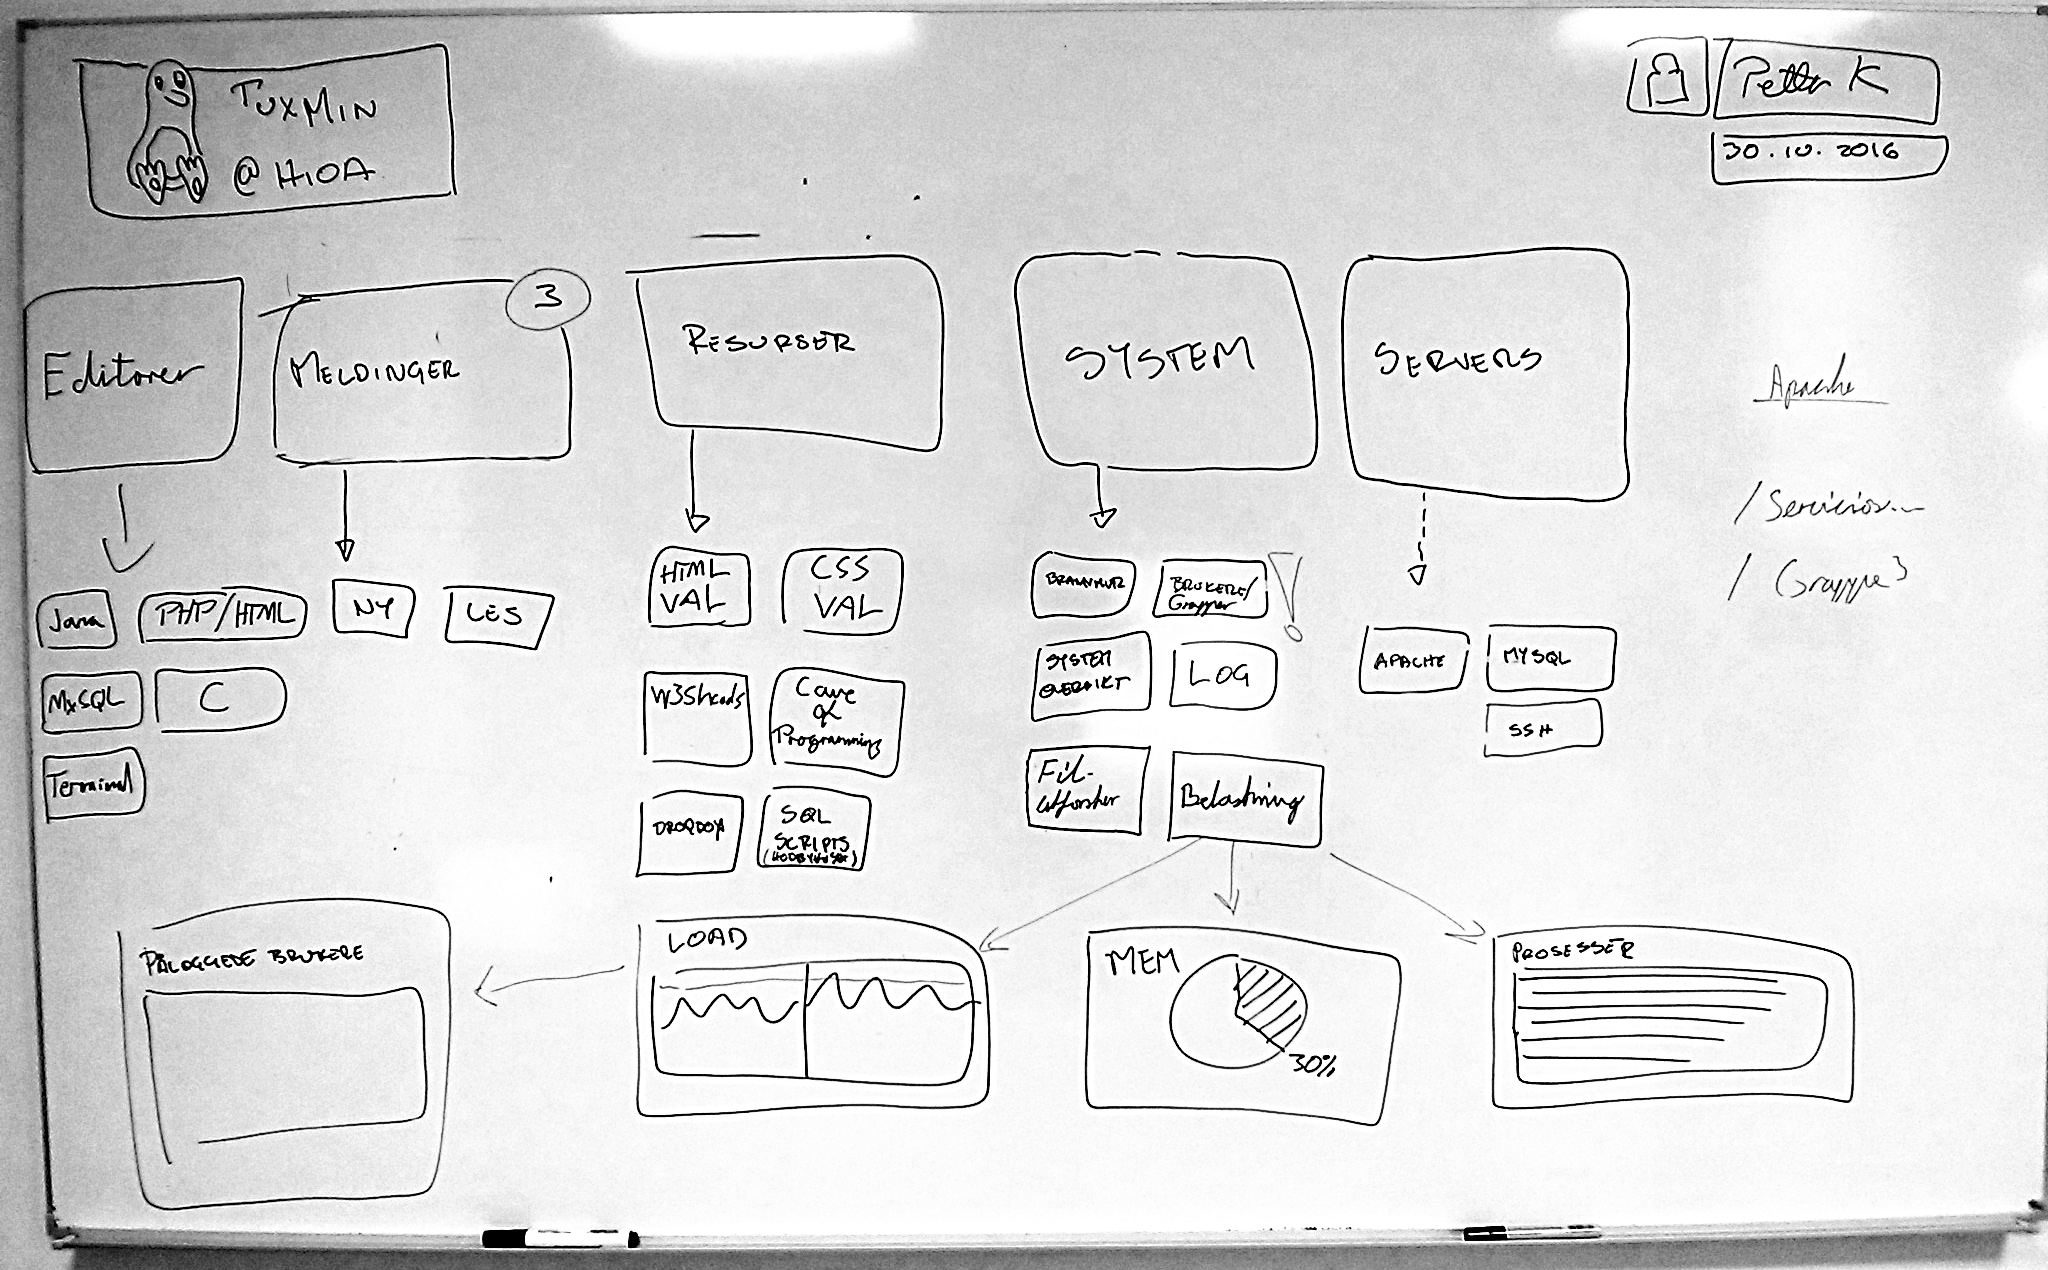
\includegraphics[width=\textwidth,height=\textheight,keepaspectratio]{./img/prosessdokumentasjon/foersteutkast/foerste.jpg}
\caption[Første utkast]{Første utkast over brukergrensesnittet.}
\label{fig:foersteutkast}
\end{figure}

\section{Low-fi prototype}
Det er ganske vanlig at man til en low-fi prototype bruker papp eller papir fo rå visualisere hvordan man kan bruke en GUI. Vi valgte å benytte oss av \href{http://balsamiq.com/products/mockups/}{balsamiq mockups} hvilket gav oss mulighet å ikke bare visualisere hvordan brukergrensesnittet skulle se ut men også legge inn enkel funksjonalitet. Slik funksjonalitet bestod av at man fikk mulighet til å klikke seg videre til neste skjermbilda fra menyer. Dette gav en ganske grei opplevelse over hvordan det kommer til å føles da man bruker produktet.

\begin{figure}
%bruk \begin{figure}[ht] dersom figuren ikke skal flyte
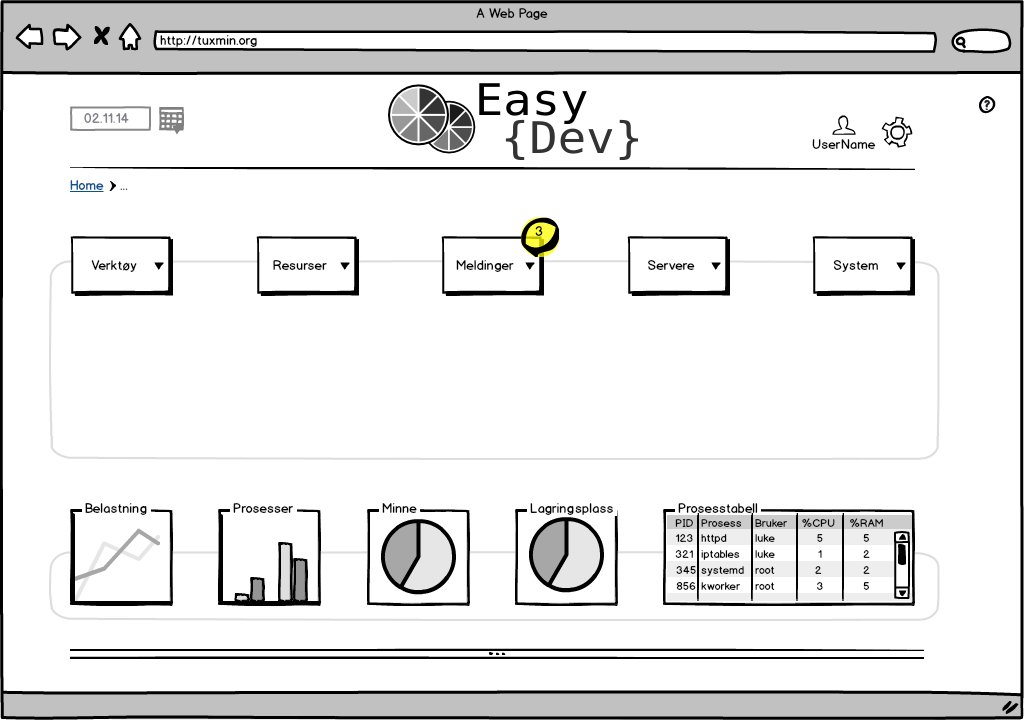
\includegraphics[width=\textwidth,height=\textheight,keepaspectratio]{./img/prosessdokumentasjon/lowfi/fremside.png}
\caption[Low-fi prototype]{Fremside for EasyDev i første low-fi prototype.}
\label{fig:lowfi_fremside}
\end{figure}

\section{Hi-fi prototype}

\section{Kriterier og avgjøresler}
Fokuser på alle valg som ble tatt. Hvilke kriterier og 
prinsipper i faget ligger bak avgjørelsene? 

Her kan vi skrive om hvorfor vi har akkuratt valgt Linux. Hvorfor skal løsningen være webbasert og hvorfor skal den kjøres i en virtuell maskin? Og så andre kriterier og avgjøresel som vi har tatt under veien. 